\chapter{获取高层支持} % Introduction chapter suppressed from the table of contents

我:对于过程改进来说,最重要的成功要素是什么?\\
客户:最难的是如何得到高层的支持,这不仅仅是嘴巴说说而已,而是要切实地给人、给时间。高层往往不清楚什么是质量改进的重点,但他们对员工的人均收入、利润(比如员工可为公司盈利的时间占比多少?如果少,就表示这个员工对公司的盈利贡献不够。)等这些财务指标都非常清楚。\\
我:非常赞同。我们可以利用评估机会来引起高层对质量改进的重视,但往往评估组只说软件开发的各种问题,难以引起他们注意。一般人,尤其是高层,一听到问题都会觉得比较烦,没有动力听下去,更不要说有对应的改进行动了。\\
客户:你说的挺有道理的。确实我们每年都会有一些评估,发现了不少问题。高层也都会参加评估会,并同意这些问题需要改进。但很多时候过后就没下文了。\\
我:质量大师Dr. JURAN
有丰富的过程改进的经验,他深知要说服高层真心投入、支持改进,就必须用高层的语言打动他们。如果与高层交流,不能把团队关注的事转化成高层关注的,就难以获得立项,做改进。

我:所以在最近的评估里,我会引导公司内部的评估组成员,通常是公司的PMO或QA,跟发起人(公司高层)汇报时,着重汇报关于如何改进、为公司节省成本的初步方案。你要兴趣听听这案例吗?\\
客户:非常有兴趣。\\
%==案例 ==
\hypertarget{ux7b2cux4e00ux7248ux65b9ux6848ux4e66}{%
\subsection{案例}\label{ux7b2cux4e00ux7248ux65b9ux6848ux4e66}}
我问公司内部评估组,高层有哪些关注点?他们就列出来,如人均收入,人均利润等商务指标。\\
然后我再问影响这些指标的因素很多,有些是软件开发团队无法控制的,例如销售人员与客户的关系,所以我们必须从这些高层关注的指标细分到一些团队实际可以影响到的指标。有哪些呢?\\
评估组:项目进度的偏差,遗漏给客户的缺陷数。\\
我:这些我们都叫性能目标。这些指标是如何影响高层目标的?\\
评估组:比如项目延误,成本就会超支。\\
我:是的。如果我们过程改进希望改善质量、减少缺陷,你们觉得会对成本有什么影响?\\
评估组:改进要投入工作量,肯定会增加成本。但长远应可能降低成本。\\
我:很多高层都不熟悉质量管理,所以很少关注和监控团队的缺陷。他们通常还是会觉得质量改进是好事,但要花成本。我做到客户满意的水平就可以了,不要追求十全十美,也正是这个误解,才导致他们认为大部分缺陷在系统测试或验收阶段才发现是正常的,是常态。如果是做软件产品的公司会好一些。我们在前面迭代回顾里面解释了,尤其在软件工程领域,因为缺陷发现越靠后,返工工作量是在前面发现的同样缺陷的几十倍。所以如果我们能把返工缺陷预先发现并处理,必然会大量降低返工工作量,与相关成本。\\

\hypertarget{ux7b2cux4e00ux7248ux65b9ux6848ux4e66}{%
\subsection{第一版方案书}\label{ux7b2cux4e00ux7248ux65b9ux6848ux4e66}}

小李做了第一版的方案书。\\
%\href{文件:方案书1.jpg}{600px}

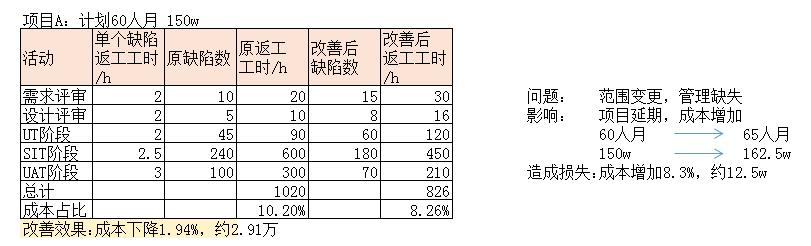
\includegraphics[width=10cm]{方案书1.jpg}

我:小李,挺好的。你在投资方面是保守型吗?\\
小李:不是啊,我还会定期买股票,因为单是靠银行定期,利息太低了。\\
我:但是看你在质量改进方面的目标很保守。比如你看,说如果做了改进以后,后面的缺陷可以降低百分之十到百分之二十,然后最后算出来节省不到五个点。你估计高层会买单,投资你这个项目吗?\\
小李:确实有道理。\\
我:你这里有几个地方没做对,例如从我们过去的经验,因为很多团队在前面几乎没做好单元测试或代码扫描,反之,系统测试或者验收测试的缺陷几乎可以减少一半。低的目标不是好目标,还有,你评估在后面阶段返工的工作量也太低了,只是比前面发现的高一点点。你尝试依据这两个思路再调一下吧。\\
小李:你有所不知
,我们虽然有些行业参考数据,但没有实际项目数据支撑,是否需要先找些实际数据才可以做方案,不然好像说不过去。\\
我:在初步方案阶段,其实不需要实际数据的支撑。你可以想象,目的是要让管理者有依据做决定,如果你想利用数据把这些数字做得更准确,这对高层的决策没有实际帮助。所以在初始阶段,合理的估算就足够了,不需要花精力在没有价值的事情上。\\

\hypertarget{ux7b2cux4e8cux7248ux4e0eux4e2dux5c42ux786eux8ba4-ux7136ux540eux5411ux9ad8ux5c42ux6c47ux62a5}{%
\subsection{第二版与中层确认,
然后向高层汇报}\label{ux7b2cux4e8cux7248ux4e0eux4e2dux5c42ux786eux8ba4-ux7136ux540eux5411ux9ad8ux5c42ux6c47ux62a5}}

做了第二版后,我们再跟中层确认一下,他们觉得这个也确实比之前更有说服力了。建议中层除了数字以外,如果能配上一些柱状图,可以让听众(高层)更容易理解。\\
%\href{文件:!!JiangJingFinal2presentScreenshot_2022-09-12_092535.jpg}{600px}

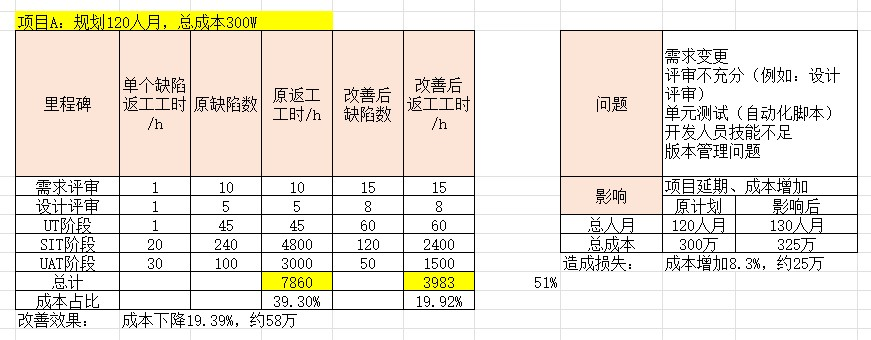
\includegraphics[width=10cm]{JiangJingFinal2presentScreenshot20220912092535.jpg}

小李跟高层汇报,并得到高层的认可后,高兴地说:以前都以为过程改进应先自己默默耕耘,先在试点取得效果,再跟高层要资源,再推广,现在看,还是应该一开始便提具体改进方案,并立项,才有机会成功。\\
我:管理层是过程改进最重要的干系人,必须一开始便得到他们支持。你后面有什么计划?\\
小李:既然他们都同意,我就开始找项目开始试点,对吗?\\
我:应该马上制定详细的计划,包括团队分工,否则你的改进方案还是难以落地。\\
小李:你说的有道理,我马上今周做,然后发他们邮件跟进。\\

\framebox{%
\begin{minipage}[t]{0.97\columnwidth}\raggedright
\hypertarget{ux53cdux9988}{%
\subsubsection{反馈}\label{ux53cdux9988}}

某CTO:
方向很好,但高层关注的不只是销售额这些商业指标,还有交付效率和质量的指标。\\
公司老板针于研发除了关注成本外,也关注:

\begin{itemize}
\tightlist
\item
  人员:人均薪资、人均产能、人员参项率(有收入的项目)、人员闲置率
\item
  进度:是否能正常交付
\item
  质量:缺陷率、严重缺陷数
\end{itemize}

举例说明:比如提升效率这样的指标,多数公司都用人均产值,人均交付金额这些指标。但大多数公司没有想过创新,如果公司业务很稳定,那么针对重复性工作是否能形成公共组件或低代码平台,来大幅度提升生产率。再说质量方面,如果客户能参与使用,例如,产品定义,需求的质量会大幅度提升(不仅依赖评审,测试)。对于这个逻辑,凡是做过程改进的人都能理解,但为什么客户不愿意深度参与,是因为没有让客户可以高效参与的工具。\\
例如,90\%以上的公司都是靠需求文档,RP原型的方式沟通需求,效率不可能高。但如果低代码平台能快速形成需求和客户可体验的需求,效率和质量都会大幅度提升。

我:
过程改进想要成功,首先必须得到高层的支持,但团队往往只关注日常任务,高层不一定懂质量,所以必须靠中层作为高层与下面团队的桥梁,把质量改善简化成高层可以理解的方案,让他决策。\\
%::\href{文件:三角形.jpg}{400px}
::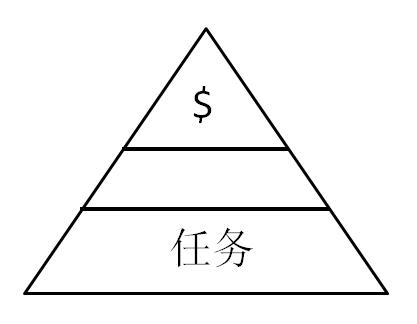
\includegraphics[width=10cm]{三角形.jpg}
上面这案例,高层只关注财务指标,没有任何质量或创新的度量指标,虽然我们都知道单靠财务指标是不全面的,但也只能用财务数据。但如果面对像你这种通情达理的高层,就可以更全面,从质量、创新等多维度估计改进可为公司带来的价值。\\
\strut
\end{minipage}}

\hypertarget{ux603bux7ed3}{%
\subsubsection{总结}\label{ux603bux7ed3}}

从以上简单案例,得到的经验教训:\\
1.评估是接触到高层最好的机会\\
2.但评估往往只是针对具体的问题,对不上高层关注的方向,难以获得实际支持\\
3.在做改进方案时,只需要估算,暂时不需要实际数据,以此可以节省资源和时间\\
4.如果确实有高层真正支持的话,就必须正式立项,再配上具体的团队、分工和详细计划,否则整个改进计划还是一纸空文\\



